% Copyright 2004 by Till Tantau <tantau@users.sourceforge.net>.
%
% In principle, this file can be redistributed and/or modified under
% the terms of the GNU Public License, version 2.
%
% However, this file is supposed to be a template to be modified
% for your own needs. For this reason, if you use this file as a
% template and not specifically distribute it as part of a another
% package/program, I grant the extra permission to freely copy and
% modify this file as you see fit and even to delete this copyright
% notice. 

\documentclass{beamer}

% There are many different themes available for Beamer. A comprehensive
% list with examples is given here:
% http://deic.uab.es/~iblanes/beamer_gallery/index_by_theme.html
% You can uncomment the themes below if you would like to use a different
% one:
%\usetheme{AnnArbor}
%\usetheme{Antibes}
%\usetheme{Bergen}
%\usetheme{Berkeley}
%\usetheme{Berlin}
%\usetheme{Boadilla}
%\usetheme{boxes}
%\usetheme{CambridgeUS}
%\usetheme{Copenhagen}
%\usetheme{Darmstadt}
\usetheme{default}
%\usetheme{Frankfurt}
%\usetheme{Goettingen}
%\usetheme{Hannover}
%\usetheme{Ilmenau}
%\usetheme{JuanLesPins}
%\usetheme{Luebeck}
%\usetheme{Madrid}
%\usetheme{Malmoe}
%\usetheme{Marburg}
%\usetheme{Montpellier}
%\usetheme{PaloAlto}
%\usetheme{Pittsburgh}
%\usetheme{Rochester}
%\usetheme{Singapore}
%\usetheme{Szeged}
%\usetheme{Warsaw}

\usepackage{setspace} 
\usepackage{amsmath}
\usepackage{graphicx}
\newcommand*{\LargerCdot}{\raisebox{-0.25ex}{\scalebox{2.3}{$\cdot$}}}

\usepackage{color}
%\input{rgb}

\definecolor{red1}{rgb}{1.000000,0.000000,0.000000}

\title{Skulls, Turbulence and Financial Markets}

% A subtitle is optional and this may be deleted
\subtitle{A study of Turbulence in Financial Markets}

\author{R.~Krishna\inst{} \and O.~Shakernia\inst{1}}
% - Give the names in the same order as the appear in the paper.
% - Use the \inst{?} command only if the authors have different
%   affiliation.

\institute[Universities of Somewhere and Elsewhere] % (optional, but mostly needed)
{
  \inst{}%
  %Summer Intern\\
  %Research Affiliates
  \and
  \inst{1}%
  Vice President Research\\
  Research Affiliates}
% - Use the \inst command only if there are several affiliations.
% - Keep it simple, no one is interested in your street address.

\date{}
% - Either use conference name or its abbreviation.
% - Not really informative to the audience, more for people (including
%   yourself) who are reading the slides online

\subject{Theoretical Computer Science}
% This is only inserted into the PDF information catalog. Can be left
% out. 

% If you have a file called "university-logo-filename.xxx", where xxx
% is a graphic format that can be processed by latex or pdflatex,
% resp., then you can add a logo as follows:

%\pgfdeclareimage[height=0.8cm]{university-logo}{ra1.png}
%\logo{\pgfuseimage{university-logo}}

% Delete this, if you do not want the table of contents to pop up at
% the beginning of each subsection:
%\AtBeginSubsection[]
%{
%  \begin{frame}<beamer>{Outline}
%    \tableofcontents[currentsection,currentsubsection]
%  \end{frame}
%}

% Let's get started
\begin{document}

\begin{frame}
  \titlepage
\end{frame}

\begin{frame}{Outline}
%	\begin{scriptsize}
	 		\tableofcontents
%  		% You might wish to add the option [pausesections]
%	\end{scriptsize}
\end{frame}

% Section and subsections will appear in the presentation overview
% and table of contents.
%\section{\small{Turbulence}}
	%\section{\small{The Concept of Financial Turbulence}}
	\section{Turbulence as a measure of Systemic risk}
	% What are the other forms of systemic risk

%\setlength\listparindent{1in}
\begin{frame}{Turbulence as a measure of Systemic risk}{}
  	\begin{itemize}
  		\item {\textbf{The Concept of Financial Turbulence} \newline
 		}
		A condition of the market in which asset prices behave \alert{uncharacteristically} from their historical fashion.These 	include:
		\begin{description}
			{$\LargerCdot$ extreme price movements, \newline $\LargerCdot$ 	decoupling of correlated assets, and \newline $\LargerCdot$ 								              			coupling of uncorrelated assets.} \newline
		\end{description} 
		\item{\textbf{Turbulence as a measure of Systemic risk} \newline}
		Ingredients of Turbulence affect the systemic risk in markets.\newline
		Turbulence can be used as an indicator of systemic risk.
  	\end{itemize}
\end{frame}


%\section{Mahalanobis Distance}
\section{Quantifying Turbulence}
\begin{frame}{Quantifying Turbulence}{}
	\begin{itemize}
		\item{\textbf{Mahalanobis Distance}}\newline
		The \alert{Mahalanobis Distance} is used to quantify Turbulence:
		$$
		d_{t} = (\mathbf{y_{t}} - \mathbf{\mu})' \mathbf{\Sigma}^{-1} (\mathbf{y_{t}} - \mathbf{\mu})
		$$ where
		$\mathbf{y_{t}}$ : vector of asset returns;\newline
		\hspace*{0.51 in}$\mathbf{\mu}$: sample average vector of asset 	returns;\newline
		\hspace*{0.485 in}$\mathbf{\Sigma}$: sample covariance matrix of asset returns;\newline
		\hspace*{0.47 in}$d_{t}$: turbulence at time $t$.
		\vspace{0.1in}
		\item{Example of a two-asset scenario:} \newline
		%$\LargerCdot$The center represents the average of \\the joint returns of assets.\newline
		$\LargerCdot$Assets equidistant by Euclidean \\measure show uncharacteristic behavior\\ with respect to the historical trends.\\
		$\LargerCdot$Equi-distance by Mahalanobis measure \\is a more accurate explanation \\of trends.    
	\end{itemize}

	\begin{figure}{}
		\vspace*{-5.0 cm}
		\scalebox{0.5}
		{\hspace*{5.7in}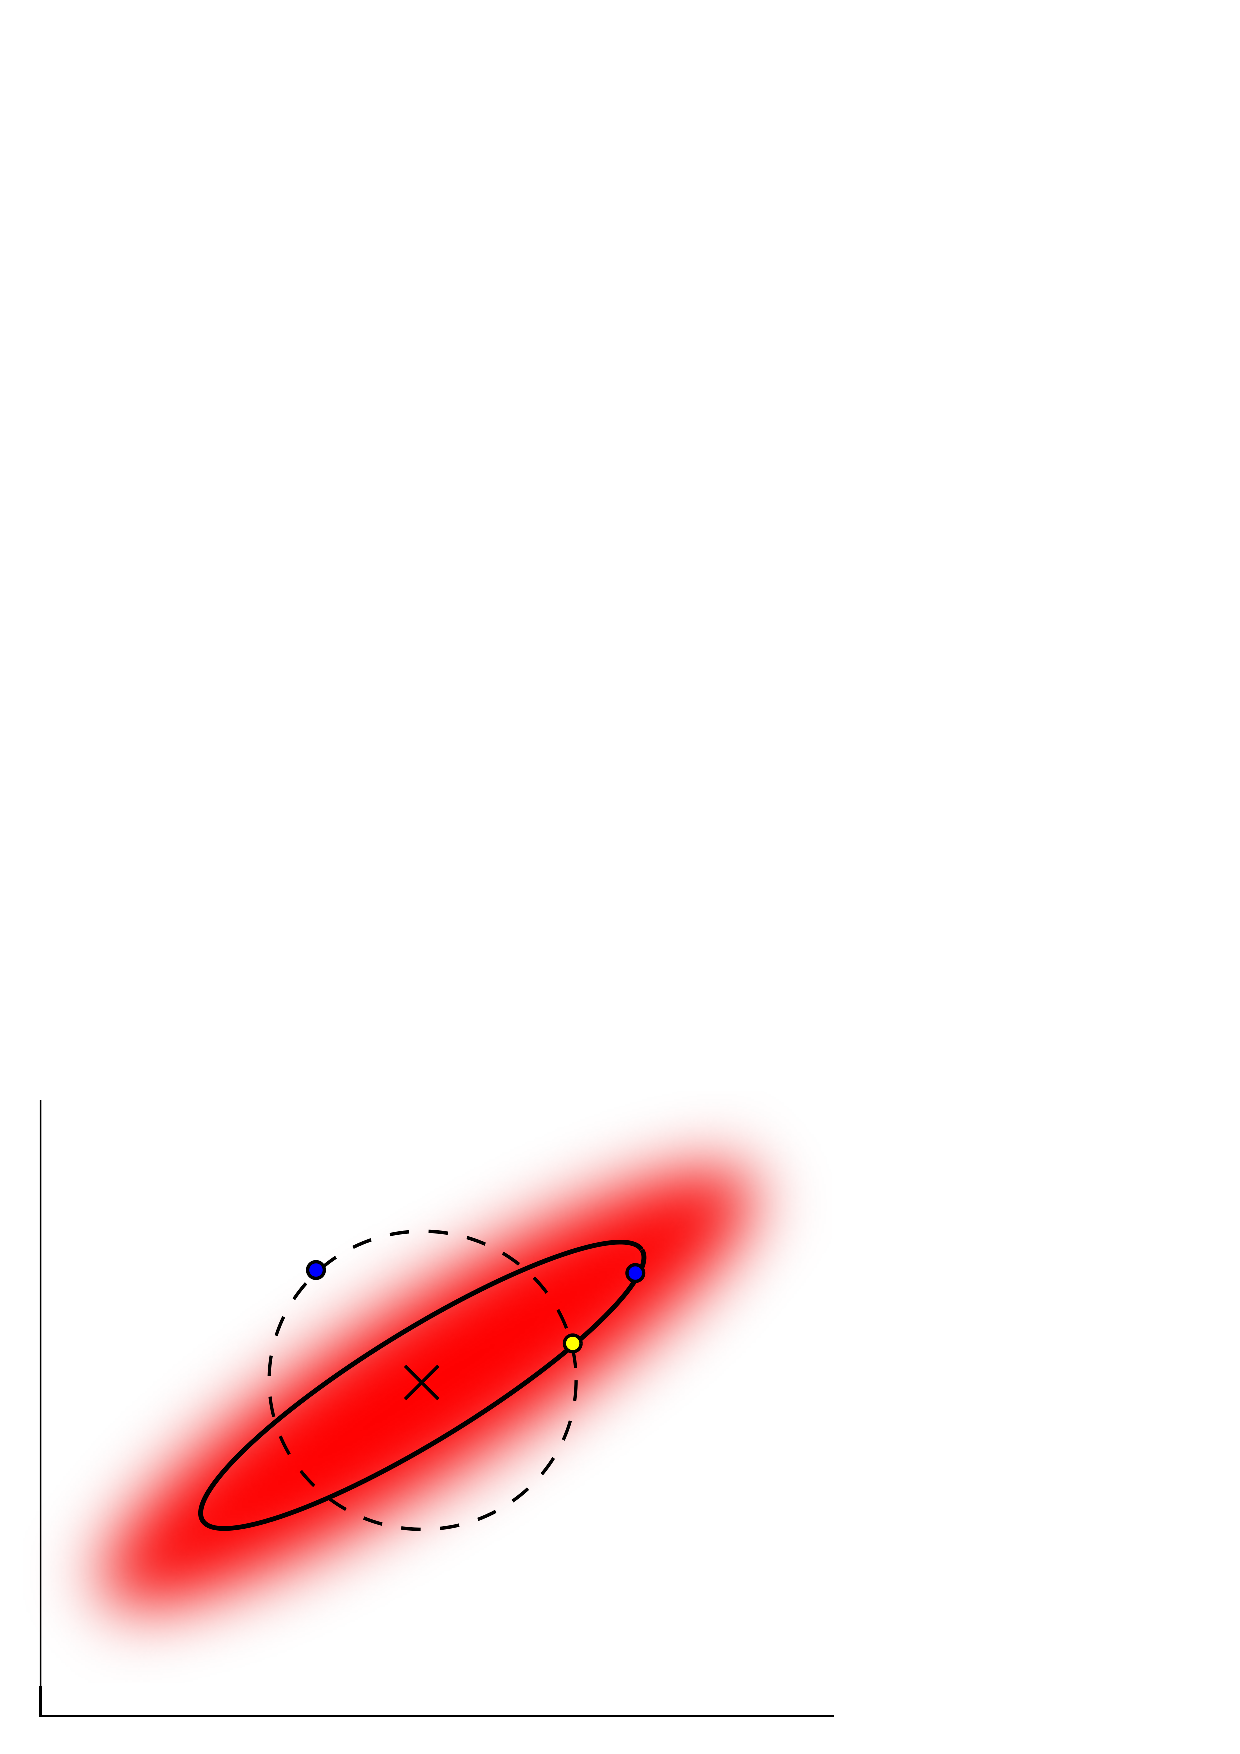
\includegraphics[scale=0.7]{fig1.pdf} }
	\end{figure}
\end{frame}


\begin{frame}{Quantifying Turbulence}{contd...}
	\begin{itemize}
		\item{We measure the Mahalanobis distance of the returns of assets 				across time.}\newline
		\item{The Covariance matrix is constructed using historical monthly returns spanning $32$ years of data ($1980 - 2012$).}\newline
		\item{This ``full-sample'' covariance matrix has a {\color{blue}look-ahead bias}.}\newline		
		\item{The distance is calculated every month using the respective monthly returns. The portfolio consists of the following assets:\newline
		$\LargerCdot$S\&P 500 TR USD \hspace*{0.59in}$\LargerCdot$MSCI EAFE GR USD\\
		$\LargerCdot$Barclays US Agg TR USD \hspace*{0.1in}$\LargerCdot$S\&P GSCI TR USD\\
		$\LargerCdot$FTSE NAREIT TR.}
	\end{itemize}
\end{frame}

%\subsection{\small{Full-sample Turbulence Index}}
\begin{frame}{Quantifying Turbulence}{contd...}
	\vspace*{-0.2 cm}
  	\begin{itemize}
		\item{\textbf{Full-sample Turbulence Index}}
		\vspace*{-0.52 cm}
		\begin{figure}
		\scalebox{0.7}
		{\hspace*{-0.23in}\includegraphics[scale=0.6]{Rplot.png} }
	\end{figure}
	\vspace*{-0.2 in}
		\item{We also examine the distances calculated using a 				Covariance matrix that does not have a look-ahead bias.}
	\end{itemize}
\end{frame}

\section{Full-sample versus ``Real-time" Turbulence Index}
\begin{frame}{Quantifying Turbulence}{contd...}
	\vspace*{-0.06 in}
  	\begin{itemize}
		\item{\textbf{``Real-time" Turbulence Index}}
		\vspace*{-0.58cm}
		\begin{figure}
			\scalebox{0.8}
			{\hspace*{-0.3in}\includegraphics[scale=0.6]{Rplot01_incep.png} }
		\end{figure}
		\vspace*{-0.5cm}
		\item{To compute the Real-time Mahalanobis distance, a covariance matrix is constructed using data up to time $t$.}
%$\LargerCdot$First $5$ years data are used to form the initial covariance matrix.\newline
	\end{itemize}
\end{frame}

%\subsection{\small{``Real-time" versus Full-sample Turbulence Index}}
\begin{frame}{Full-sample versus ``Real-time" Turbulence Index}{contd...}
 	\begin{itemize}
	\vspace*{-0.1 in}
		\item{\textbf{``Real-time" versus Full-sample Turbulence Index}}
		\vspace*{-0.25 in}
		\begin{figure}
			\scalebox{0.65}
			{\hspace*{-0.5in}\includegraphics[scale=0.6]{mod(blue)VsOri(black).pdf} }
		\end{figure}
	\vspace*{-0.3cm}
		\item{We examine the performance of using the Real-time covariance matrix to asses turbulence in markets.}
	\end{itemize}
\end{frame}

%\subsection{\small{Distinguishing Turbulent and Calm periods}}
\begin{frame}{Full-sample versus ``Real-time" Turbulence Index}{contd...}
	\vspace*{0 in}
	\begin{itemize}
		\item{\textbf{Distinguishing Turbulent and Calm periods}}\vspace{0in}
		\item {New information on returns causes changes in Mahalanobis distances compared to the 			historical patterns observed.}\newline
		\item {This variance is exploited to identify Calm and Turbulent periods.} \newline
		\item{Returns that incur large deviations from the historical mean and/or historical correlations yield large distances.}\newline
		\item {A measure of \alert{$75$ percentile} of Mahalanobis distance is used to distinguish between Calm and Turbulent periods.}
	\end{itemize}
\end{frame}

%\subsection{\small{Performance of the Real-time Turbulence measure}}
\begin{frame}{Full-sample versus ``Real-time" Turbulence Index}{contd...}
	\vspace*{-0.2 in}
	\begin{itemize}
		\vspace{-0 in}
		\item{\textbf{Performance of the Real-time Turbulence measure.}}
		\vspace{-0.9 in}
		\begin{figure}
			\scalebox{1}
			{\hspace*{-0.5 in}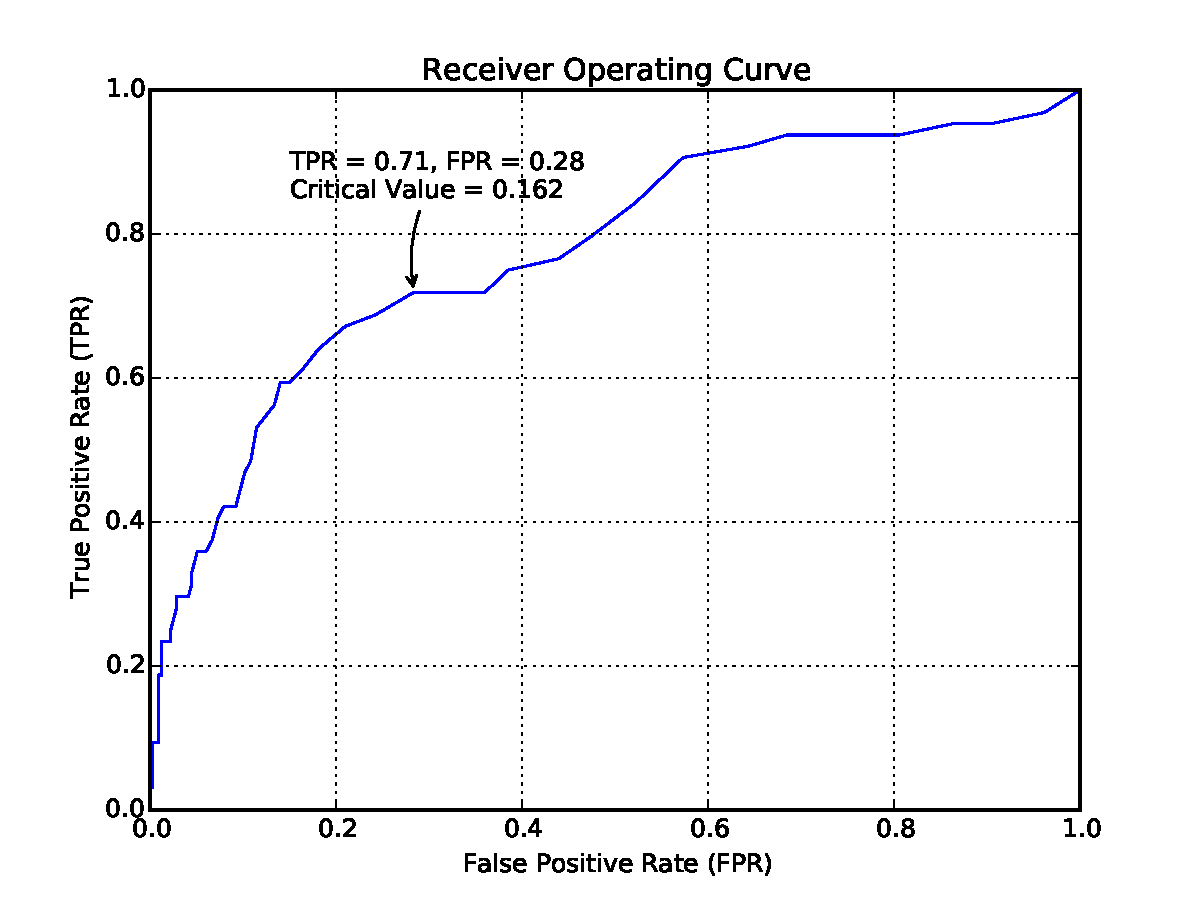
\includegraphics[scale=1]{ROC.pdf} }
		\end{figure}
	\vspace*{-9.2in}
		%\item{The performance of the Real-time Mahalanobis distance measure is established by analysing its accuracy in identifying turbulent returns from non-turbulent, or ``Calm", returns.}
		\item{The comparison shows a False Negative rate of $3$\%; and a False Positive rate of $17$\%.}
	\end{itemize}
\end{frame}

\section{\small{Turbulence in Portfolios and in Asset Classes}}
%\subsection{\small{The effect of Turbulence in Asset Classes}}
\begin{frame}{Turbulence in Portfolios and in Asset Classes}{Asset Classes}
\begin{itemize}
\vspace{-1.77 in}
\item{\textbf{The effect of Turbulence in Asset Classes.}}
\vspace{-0.72 in}
\begin{figure}
	\scalebox{0.68}
	{\hspace*{-0.9in}\includegraphics[scale=1]{avRetVolCorrHTRT_assets.pdf} }
\end{figure}
\vspace*{-6.95in}
\end{itemize}
\end{frame}

\begin{frame}{Turbulence in Portfolios and in Asset Classes}{Asset Classes}
\begin{itemize}
\vspace*{-0in}
\item{The effect of Turbulence in Asset classes over time.}
\begin{figure}
\begin{itemize}
\begin{center}
	\vspace*{-0.2in}
	\hspace*{-0.9in}
	\includegraphics[width=0.57\textwidth]{assetClassVariance3.pdf} 
    \includegraphics[width=0.57\textwidth]{assetClassVariance2.pdf} 
\end{center}
\end{itemize}
\end{figure}
\end{itemize}
\end{frame}

%\begin{frame}{Turbulence in Portfolios and in Asset Classes}{Asset Classes}
%	\vspace*{-0.5cm}
%	\begin{itemize}
%		\item{The average returns of assets decrease  during periods of Turbulence.}\newline
%		
%		\item{Except for Aggregate Bonds, which display the investor sentiment of {\color{blue}flight-to-safety} during turbulent times.}\newline
%		\item{Despite increase in volatility during 					Turbulence, there is a decrease in the average returns of 							assets.}\newline
%		\item{The Total Average Correlation (the sum of correlation 			values across assets) increases during periods of 						Turbulence.}\newline
%	\end{itemize}
%\end{frame}

\begin{frame}{Turbulence in Portfolios and in Asset Classes}{Asset Classes}
	\begin{itemize}
		\vspace*{0in}
		\item{Correlations across assets during Turbulent and Clam periods.}
		\vspace*{-0.55in}
		\begin{figure}
			\scalebox{0.8}
			{\hspace*{-1in}\includegraphics[scale=0.8]{avRetVolCorr_assets_trial.pdf}}
		\end{figure}
	\end{itemize}
\end{frame}

%\begin{frame}{Turbulence in Portfolios and in Asset Classes}{Asset Classes}
%	\vspace*{-0.5cm}
%	\begin{itemize}
%		\item{Increase in correlations between asset classes during turbulence, with an exception of the correlation between MSCI EAFE 				and S\&P GSCI.}\newline
%		\item{Real-time covariance matrix captures the trends in correlations seen using the Full-sample covariance matrix.}\newline
%	\end{itemize}
%\end{frame}

%\begin{frame}{Turbulence in Portfolios and in Asset Classes}{Asset Classes}
%\begin{itemize}
%\vspace*{0in}
%\item{Correlations across assets during Turbulent and Clam periods.}
%\vspace*{-0.55in}
%\begin{figure}
%	\scalebox{0.8}
%	{\hspace*{-1in}\includegraphics[scale=0.8]{corrTableTurbVsCalm_assets.pdf}}
%\end{figure}
%\end{itemize}
%\end{frame}

%\subsection{\small{The effect of Turbulence in Portfolios}}
\begin{frame}{Turbulence in Portfolios and in Asset Classes}{Portfolios}
\begin{itemize}
\vspace*{0in}
\item{\textbf{The effect of Turbulence in Portfolios}}
\vspace*{-0.73in}
\begin{figure}
	\scalebox{0.8}
	{\hspace*{-0.7in}\includegraphics[scale=1]{Table2.pdf} }
\end{figure}
\vspace*{-6.43in}
\item{The Full-sample risk was estimated from the full-sample covariance matrix, i.e. from the monthly returns during the 30-year period.}
\item{Turbulence-risk was estimated using the covariance matrix of the turbulent subsample.}
\end{itemize}
\end{frame}

\begin{frame}{Turbulence in Portfolios and in Asset Classes}{Portfolios}
	\begin{itemize}
		\vspace*{-0in}
		\item{The effect of Turbulence in Portfolios over time.}
		\begin{figure}
			\begin{itemize}
				\begin{center}
					\vspace*{0.1in}
					\hspace*{-0.8in}
	                  \includegraphics[width=0.51\textwidth]{portfolioVariance1.pdf} \hspace{0.02in}
                       \includegraphics[width=0.51\textwidth]{portfolioVariance2.pdf} 
				\end{center}
			\end{itemize}
		\end{figure}
		\hspace*{-0.5in}
		\parbox{5in}{$\LargerCdot$Volatility for the first 5-years is calculated using a forward-looking\\ covariance matrix; the rest are computed using the ``Real-time''\\ covariance matrix.}\newline
%$\LargerCdot$A single Turbulence threshold value is calculated for the first 5-years. Turbulent and Calm returns were identified using new thresholds realised at every time instant.}
	\end{itemize}
\end{frame}

\section{Turbulence Resistant Portfolios}
\begin{frame}{Turbulence Resistant Portfolios}{}
	\begin{itemize}
		\item{The purpose of quantifying turbulence in markets is \alert{not} to forecast the occurrence of turbulence in markets.}\newline
		\item{The aim is to develop tools and techniques to build portfolios that are resistant to turbulence in markets.}\newline  
		\item{A turbulence resistant portfolio (\alert{robust portfolio}) would have higher returns than a non-resistant portfolio during turbulence.}\newline
		\item{The trade-off of ensuring higher returns during turbulence is the realisation of marginally lower returns during calm 							periods.}\newline
		\item{Marginal under performance behaves as a \alert{premium} paid for the out 				performance of the robust portfolio during turbulence}
	\end{itemize}
\end{frame}

%\subsection{\small{Building Turbulence Resistant Portfolios}}
\begin{frame}{Turbulence Resistant Portfolios}{contd...}
	\begin{itemize}
		\item{\textbf{Building Turbulence Resistant Portfolios}}
		\item{Difference in the properties of the \alert{covariance matrix} and of the \alert{vector of mean} returns during turbulent and calm periods are exploited.} 
		%are exploited in constructing robust portfolios.}
		\item{The robust portfolio is built using the following steps: \newline
		$\LargerCdot$ Using the Mahalanobis distance measure, historical return of assets is partitioned into turbulent and calm.\\
		$\LargerCdot$ The covariance matrix of the robust portfolio is constructed:
	\begin{figure}{}
		\vspace*{-0.06 in}
		\scalebox{0.45}
		{\hspace*{0.6 in}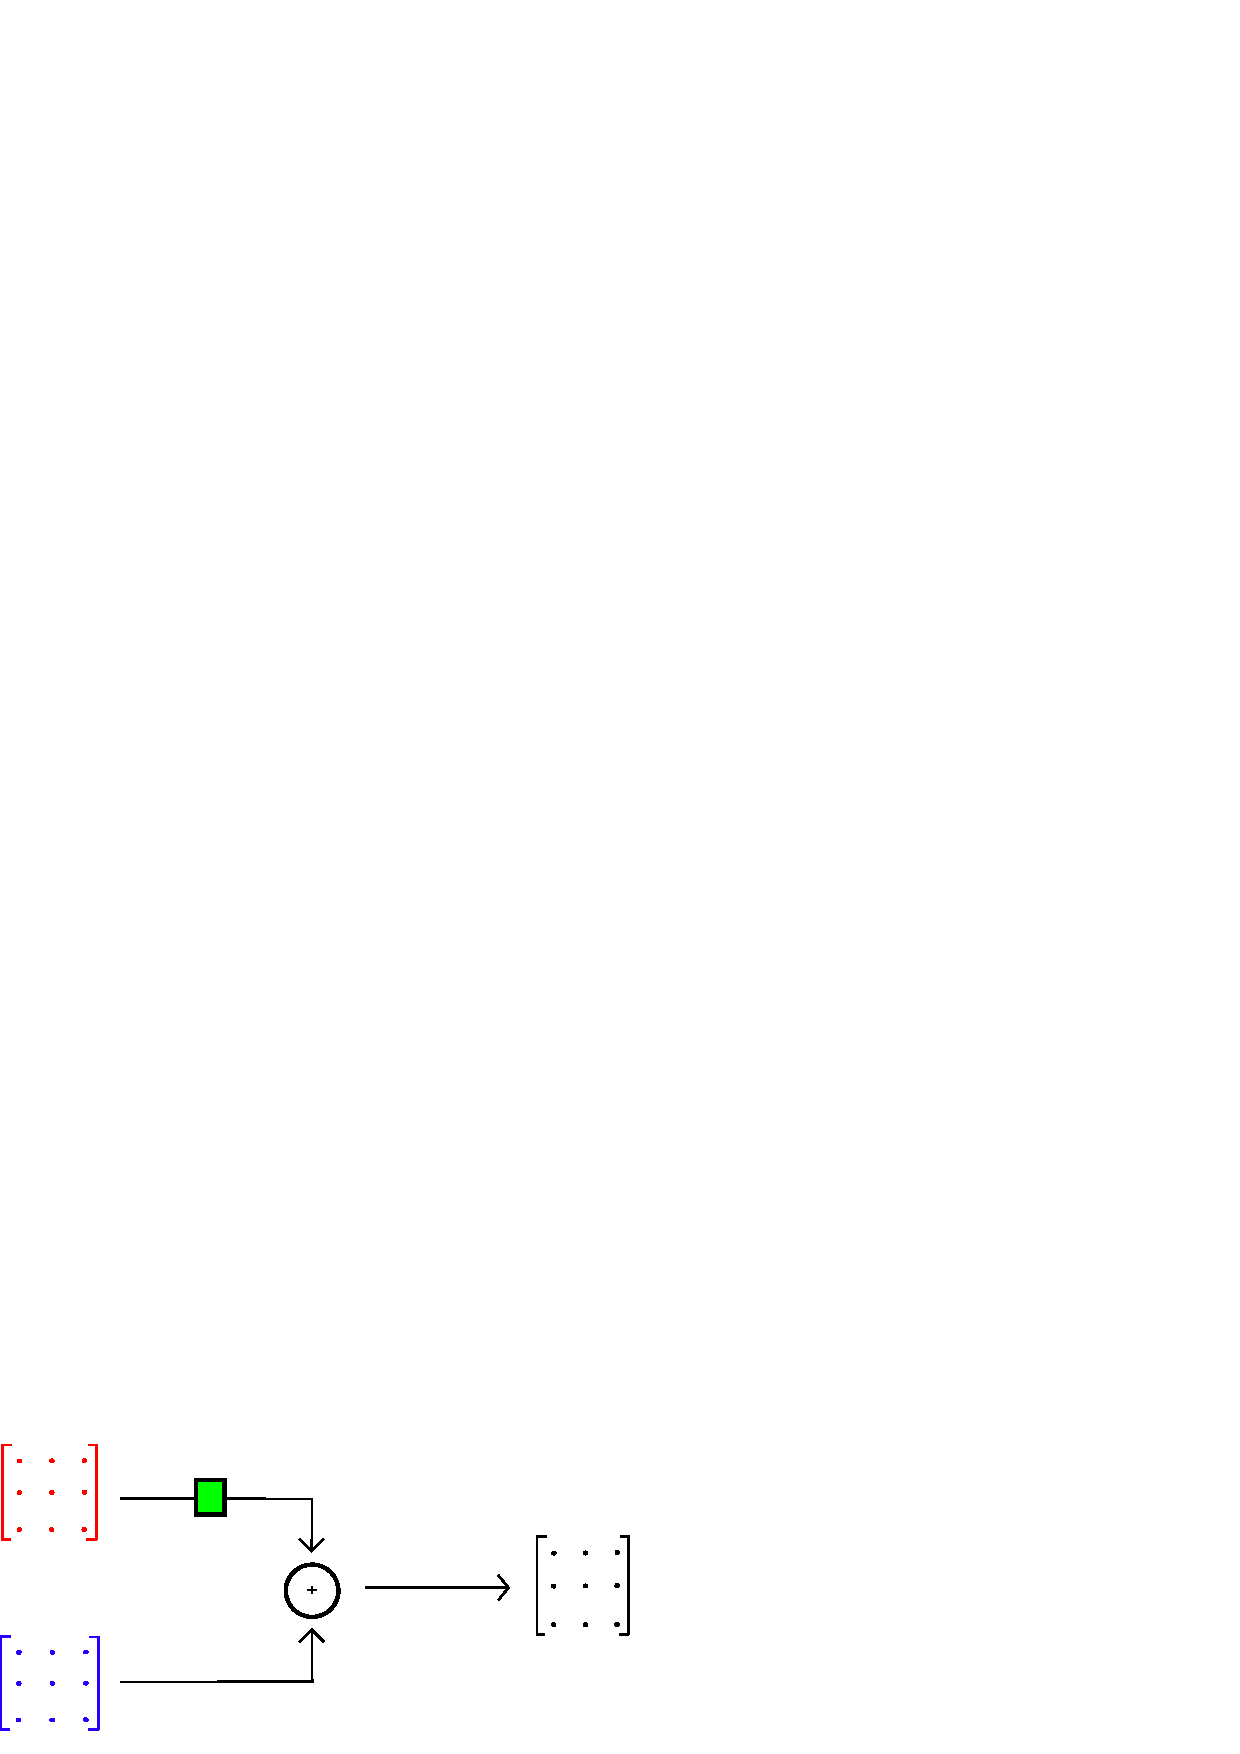
\includegraphics[scale=0.9]{fig2.png} }
	\end{figure}
	\vspace*{-0.05 in}
	where $c = \frac{\text{no. turbulent returns}}  {\text{no. non-turbulent returns}}$.
}
\end{itemize}
\end{frame}

\begin{frame}{Turbulence Resistant Portfolios}{contd...}
	$\LargerCdot$ The mean of returns of the robust portfolio are designed: 
	\begin{figure}{}
		\vspace*{-0.1 in}
		\scalebox{0.5}
		{\hspace*{0 in}\includegraphics[scale=0.9]{fig3.png} }
	\end{figure}
	\vspace*{-0.3 in}
	where,$$w = \frac{n + 2}{n + 2 + T \big( \mathbf{\hat{\mu}} - \mathbf{\mu_m} \mathbf{e}\big)^{T} \mathbf{\Sigma^{-1}}\big( 			\mathbf{\hat{\mu}} - \mathbf{\mu_m} \mathbf{e}\big)}$$
	$n$ is the number of assets, $T$ is the sample size and $\mathbf{\Sigma}$ is \\the sample covariance matrix.
\end{frame}

\begin{frame}{Turbulence Resistant Portfolios}{contd...}
	$\LargerCdot$The ``Equilibrium returns" are derived using a reverse optimization method using the mean-variance optimization framework:
\vspace*{-0.1in}
$$
		\mathbf{\mu_{equi.}} = \lambda \Sigma \mathbf{w_{mkt.}}
$$ where $\mathbf{\mu_{equi.}}$ is the Implied Equilibrium returns,\newline
\hspace*{0.35 in}$\lambda$ is the risk-aversion coefficient,\newline
\hspace*{0.35 in}$\Sigma$ is the covariance matrix of excess returns, and\newline
\hspace*{0.35 in}$\mathbf{w_{mkt.}}$ is the market-clearing portfolio weight.\newline

$\LargerCdot$The risk-aversion coefficient  can be estimated as
$$
	\lambda = \frac{E(r) - r_f}{\sigma^2}
$$
where $E(r)$ is the expected market return, $r_f$ is the risk-free rate, and $\sigma$ is chosen to be $10\%$.  

$\LargerCdot$The portfolio was made up of: MSCI EAFE, S\&P GSC, FTSE NAREIT, {\color{blue}{Barclays US Treasury Long, S\&P 500}} {\color{black}{and}} \\ {\color{blue}{Barclays US Agg}}.

\end{frame}

\begin{frame}{Turbulence Resistant Portfolios}{contd...}
	%\parbox{5in}{$\LargerCdot$The robust-portfolio is then identified in the mean-variance \\framework by using the expected returns and the covariance matrix.}
	\vspace*{-0.6in}
	\begin{itemize}
		\item{The performance of the robust and non-robust portfolios were compared using the following simulation framework:}\newline\\
$\LargerCdot$Divide sample space of historical returns \\randomly into two equal halves: \\{\color{blue}training space} - to build the portfolios, and \\{\color{blue}testing space} - to test their performance.\newline\\
		$\LargerCdot$Turbulent returns in the training space were \\ identified using a \alert{70 percentile} threshold.\newline\\
	    $\LargerCdot$Threshold of the training space is used to\\ identify turbulent and calm returns in the testing space.\newline\\
$\LargerCdot$This was repeated 1000 times and the performance was evaluated across the iterations. 
				\begin{figure}{}
			\vspace*{-2.7 in}
			\scalebox{0.5}
			{\hspace*{6.2 in}\includegraphics[scale=0.8]{fig4.png} }
		\end{figure}
	\end{itemize}
\end{frame}

%\subsection{\small{Simulation Results}}
\begin{frame}{Turbulence Resistant Portfolios}{contd...}
	\begin{itemize}
	\vspace*{-0.1in}
		\item{\textbf{Simulation Results}}
		\begin{figure}
			\vspace*{-0.6 in}
			\scalebox{0.7}
			{\hspace*{-1.2 in}\includegraphics[scale=0.89]{testSummary1.pdf} }
		\end{figure}
%		\vspace*{-5.5 in}\hspace*{2.4in}
%		\parbox{1.8in}{$\LargerCdot${\color{blue}Sub-sample gain}: Difference in median of robust and non-robust portfolios during Turbulent periods.\newline\\
%		$\LargerCdot${\color{red}Full-sample cost}: Under performance of robust portfolio across full-sample.}
		\end{itemize}
\end{frame}

\begin{frame}{Turbulence Resistant Portfolios}{contd...}
$\LargerCdot$ Box plots of realised weights of robust and non-robust portfolios.
\vspace*{-0.4 in}
	\begin{figure}
		\begin{itemize}
			\begin{center}
				\vspace*{0in}
				\hspace*{-0.75in}
		 	    \scalebox{0.75}{
				\includegraphics[width=0.8\textwidth]{turbRobPortPlotA.pdf} \hspace{0 in}
    				\includegraphics[width=0.8\textwidth]{turbRobPortPlotB.pdf} }
			\end{center}
		\hspace*{-0.5in}
		$\LargerCdot$A substantially higher proportion of weights were allocated to \\\hspace*{-0.37in}{\color{blue}Barclays US Treasury Long, S\&P 500 and Barclays US Agg.}
		\end{itemize}
	\end{figure}
\end{frame}

%\begin{frame}{Turbulence Resistant Portfolios}{contd...}
%$\LargerCdot$ Box plots of realised volatility of robust and non-robust portfolio.
%\vspace*{-0.4 in}
%	\begin{figure}
%		\begin{itemize}
%			\begin{center}
%				\vspace*{0in}
%				\hspace*{-0.75in}
%		 	    \scalebox{0.75}{
%				\includegraphics[width=0.8\textwidth]{turbRobPortPlotC.pdf} \hspace{0 in}
%    				\includegraphics[width=0.8\textwidth]{turbRobPortPlotD.pdf} }
%			\end{center}
%		\end{itemize}
%	\end{figure}
%\end{frame}

%\begin{frame}{Turbulence Resistant Portfolios}{contd...}
%$\LargerCdot$ Box plots of realised returns of robust and non-robust portfolio. 
%\vspace*{-0.4 in}
%	\begin{figure}
%		\begin{itemize}
%			\begin{center}
%				\vspace*{0in}
%				\hspace*{-0.75in}
%		 	    \scalebox{0.75}{
%				\includaegraphics[width=0.8\textwidth]{turbRobPortPlotE.pdf} \hspace{0 in}
%    				\includegraphics[width=0.8\textwidth]{turbRobPortPlotF.pdf} }
%			\end{center}
%		\end{itemize}
%	\end{figure}
%\end{frame}

\section{Turbulence and Business Cycles}
\begin{frame}{Business Cycles}{}
		\vspace*{-0.3 in}
		\begin{figure}
			\scalebox{0.7}
			{\hspace*{-0.4in}\includegraphics[scale=0.55]{turbRecSlow.pdf}}
		\end{figure}
		\vspace*{-0.4 in}
		\begin{itemize}
			\item{We observe that periods of Turbulence coincide with Business Cycles such as Recession-Expansion and Growth-Slow downs.}
		\end{itemize}
\end{frame}

%\subsection{\small{Turbulent robust portfolios in Growth Cycles}}
\begin{frame}{Business Cycles}{contd...}
		\vspace*{-0 in}
		\begin{itemize}
		\item{\textbf{Turbulence robust portfolios in Growth-Slow down periods.}}
		\vspace*{-0.71in}
		\begin{figure}
			\scalebox{0.72}
			{\hspace*{-0.6in}\includegraphics[scale=0.8]{growthSummary.pdf}}
		\end{figure}
		\vspace*{-0.4 in}
	\end{itemize}
\end{frame}

%\subsection{\small{Turbulent robust portfolios in Recession Cycles}}
\begin{frame}{Business Cycles}{contd...}
		\vspace*{-0 in}
		\begin{itemize}
		\item{\textbf{Turbulence robust portfolios in Recession-Expansion periods.}}
		\vspace*{-0.71in}
		\begin{figure}
			\scalebox{0.72}
			{\hspace*{-0.6in}\includegraphics[scale=0.8]{recessionSummary.pdf}}
		\end{figure}
		\vspace*{-0.4 in}
	\end{itemize}
\end{frame}

\section{Conclusion}
\begin{frame}{Conclusion}{}
		\vspace*{-0 in}
		\begin{itemize}
			\item{Mahalanobis distances can be used to examine dislocations in correlations and changes in deviations from historic patterns.}
			\item{``Real-time'' covariance matrix captures the true trends of changes in asset returns and volatilities during turbulence.}
			\item{During Turbulence assets have high volatility and a sharp decrease in returns. The notion of flight to safety is observed.}
			\item{A general decrease in cross-correlations between assets is also observed during turbulence.}
			\item{Portfolios can be designed to withstand turbulence. An attempt was made to replicate their performance.}
			\item{Portfolios robust to turbulence tend to withstand Business Cycles of Growth-Slow downs and Recession-Expansions.} 
			%\item{The performance of robust portfolios during periods of Recession seems useful.}
	\end{itemize}
\end{frame}


\begin{frame}{}{}
	\vspace*{0.6in}
	\hspace*{1.6in}\textbf{\Large{\Large{Thank you.}}}
\end{frame}

\begin{frame}{}{}
	\vspace*{-0.06 in}
  	\begin{itemize}
		\item{\textbf{``Moving-Window" Turbulence Index}}
		\vspace*{-0.58cm}
		\begin{figure}
			\scalebox{0.5}
			{\hspace*{-0.3in}\includegraphics[scale=0.6]{movingWindow.png} }
		\end{figure}
		\vspace*{-0.5cm}
		\item{To compute the Real-time Mahalanobis distance, a covariance matrix is constructed using data up to time $t$.}
%$\LargerCdot$First $5$ years data are used to form the initial covariance matrix.\newline
	\end{itemize}
\end{frame}

\begin{frame}{}{}
	\vspace*{-0.2 in}
	\begin{itemize}
		\vspace{-0 in}
		\item{\textbf{Performance of the Moving-Window Turbulence measure.}}
		\vspace{-1.4 in}
		\begin{figure}
			\scalebox{1}
			{\hspace*{-1.5 in}\includegraphics[scale=1]{confusionMatrix.pdf} }
		\end{figure}
	\vspace*{-8.2in}
		%\item{The performance of the Real-time Mahalanobis distance measure is established by analysing its accuracy in identifying turbulent returns from non-turbulent, or ``Calm", returns.}
		\item{The comparison shows a False Negative rate of $55$\%; and a False Positive rate of $0$\%.}
	\end{itemize}
\end{frame}


% ******************************** EXTRA FEATURES **********************************
%
%% You can reveal the parts of a slide one at a time
%% with the \pause command:
%\begin{frame}{Second Slide Title}
%  \begin{itemize}
%  \item {
%    First item.
%    \pause % The slide will pause after showing the first item
%  }
%  \item {   
%    Second item.
%  }
%  % You can also specify when the content should appear
%  % by using <n->:
%  \item<3-> {
%    Third item.
%  }
%  \item<4-> {
%    Fourth item.
%  }
%  % or you can use the \uncover command to reveal general
%  % content (not just \items):
%  \item<5-> {
%    Fifth item. \uncover<6->{Extra text in the fifth item.}
%  }
%  \end{itemize}
%\end{frame}
%

%
%\begin{frame}{Blocks}
%\begin{block}{Block Title}
%You can also highlight sections of your presentation in a block, with it's own title
%\end{block}
%\begin{theorem}
%There are separate environments for theorems, examples, definitions and proofs.
%\end{theorem}
%\begin{example}
%Here is an example of an example block.
%\end{example}
%\end{frame}
%
%\subsection{Performance Analysis}
%\subsection{Shrinkage of the Covariance matrix}
%\begin{frame}{Blocks}
%\begin{block}{Block Title}
%You can also highlight sections of your presentation in a block, with it's own title
%\end{block}
%\begin{theorem}
%There are separate environments for theorems, examples, definitions and proofs.
%\end{theorem}
%\begin{example}
%Here is an example of an example block.
%\end{example}
%\end{frame}
%
%% Placing a * after \section means it will not show in the
%% outline or table of contents.
%\section*{Summary}
%
%\begin{frame}{Summary}
%  \begin{itemize}
%  \item
%    The \alert{first main message} of your talk in one or two lines.
%  \item
%    The \alert{second main message} of your talk in one or two lines.
%  \item
%    Perhaps a \alert{third message}, but not more than that.
%  \end{itemize}
%  
%  \begin{itemize}
%  \item
%    Outlook
%    \begin{itemize}
%    \item
%      Something you haven't solved.
%    \item
%      Something else you haven't solved.
%    \end{itemize}
%  \end{itemize}
%\end{frame}
%
% ******************************************

% All of the following is optional and typically not needed. 
%\appendix
%\section<presentation>*{\appendixname}
%\subsection<presentation>*{For Further Reading}
%
%\begin{frame}[allowframebreaks]
%  \frametitle<presentation>{For Further Reading}
%    
%  \begin{thebibliography}{10}
%    
%  \beamertemplatebookbibitems
%  % Start with overview books.
%
%  \bibitem{Author1990}
%    A.~Author.
%    \newblock {\em Handbook of Everything}.
%    \newblock Some Press, 1990.
% 
%    
%  \beamertemplatearticlebibitems
%  % Followed by interesting articles. Keep the list short. 
%
%  \bibitem{Someone2000}
%    S.~Someone.
%    \newblock On this and that.
%    \newblock {\em Journal of This and That}, 2(1):50--100,
%    2000.
%  \end{thebibliography}
%\end{frame}


\end{document}